% !TeX program = lualatex

\documentclass[a4paper]{article}

% Expanded on 2022-03-21 at 10:12:40.

\usepackage{../../style}

\title{Analyse 2}
\author{Joachim Favre}
\date{Lundi 21 mars 2022}

\begin{document}
\maketitle

\lecture{9}{2022-03-21}{Ça devient limite là}{
\begin{itemize}[left=0pt]
    \item Définition des fonctions réelles de plusieurs variables réelles.
    \item Définition de la notion de voisinage, de limite et de continuité pour les fonctions réelles à plusieurs variables réelles.
    \item Démonstration du théorème de la caractérisation des limites à partir des suites convergentes.
\end{itemize}

}

\section{Fonctions réelles de plusieurs variables réelles}
\subsection{Définitions et exemples}
\begin{parag}{Définition}
    Soit $E \subset \mathbb{R}^n$ un sous-ensemble non-vide où $n \geq 1$.

    Une \important{fonction} $E \mapsto \mathbb{R}^n$ est une application qui envoie chaque point $\bvec{x} = \begin{pmatrix} x_1 & \ldots & x_n \end{pmatrix} \in E$ dans $\mathbb{R}$. $E$ est \important{le domaine de définition} de $f$, et $f\left(E\right) \subset \mathbb{R}$ est \important{l'ensemble image}.
\end{parag}

\begin{parag}{Exemple 1}
    Prenons la fonction suivante: 
    \[f\left(x, y\right) = \sqrt{1 - \left(x^2 + y^2\right)}\]

    Pour notre domaine de définition, on veut que $x^2 + y^2 \leq 1$, ce qui est un disque de rayon 1 et centre $\left(0,0\right)$. Donc: 
    \[E = \left\{\left(x, y\right) \subset \mathbb{R}^2 \telque x^2 + y^2 \leq 1\right\}\]
    
    Considérons le graphique de $z = f\left(x, y\right)$. Cette équation est équivalente à:
    \[\begin{systemofequations} z^2 = 1 - \left(x^2 + y^2\right) \iff x^2 + y^2 + z^2 = 1 \\ z \geq 0 \end{systemofequations}\]
    
    Il est donc clair que c'est une hemisphère de rayon $1$ et centre $\left(0, 0, 0\right) \in \mathbb{R}^3$.
\end{parag}

\begin{parag}{Exemple 2}
    Prenons maintenant la fonction suivante: 
    \[f\left(x, y\right) = 2x + 1 \iff z = 2x + 1\]
    
    Si on considère seulement le graphique sur $x$ et $z$, alors c'est une droite. Si maintenant on rajoute $y$, on prolonge cette droite, ce qui nous donne un plan.

    \begin{center}
    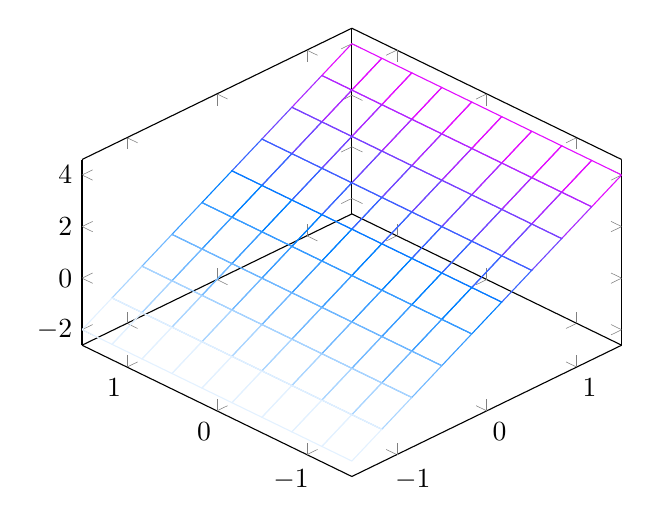
\begin{tikzpicture}
        \begin{axis}[
            view={-45}{45}
        ]
        \addplot3[
            mesh,
            samples=10,
            domain=-1.5:1.5,
            colormap/cool,
        ]
        {2*x + 1};
        \end{axis}
    \end{tikzpicture}
    \end{center}
\end{parag}

\begin{parag}{Exemple 3}
    Soient $a, b, c \in \mathbb{R}$, et la fonction suivante:
    \[f\left(x, y\right) = ax + by + c\]
    
    Clairement, $E = \mathbb{R}^2$. Nous nous demandons ce que représente cette fonction graphiquement. 

    Pour simplifier, prenons $c = 0$. Nous pouvons considérer le graphique de $f$:
    \begin{multiequality}
    F =\ & \left\{\left(x, y, z\right) \in \mathbb{R}^3 \telque ax + by = z\right\} \\
    =\ & \left\{\left(x, y, z\right) \in\mathbb{R}^3 \telque ax + by - z = 0\right\} \\
    =\ & \left\{\left(x, y, z\right) \in \mathbb{R}^3 \telque \left<\left(x, y, z\right), \left(a, b, -1\right)\right> = 0\right\} 
    \end{multiequality}
    ce qui est le plan orthogonal à $\bvec{n} = \left(a, b, -1\right)$ et qui contient $\left(0, 0, 0\right)$.

    Considérons maintenant $c \in \mathbb{R}$. Il suffit de monter le plan par $c$ unités le long de l'axe $z$ pour obtenir le graphique de notre fonction: le plan orthogonal à $\bvec{n} = \left(a, b, -1\right)$ qui contient $\left(0, 0, c\right)$.
\end{parag}

\begin{parag}{Définition}
    Soit $f : E \mapsto \mathbb{R}^n$ et $c \in f\left(E\right) \subset \mathbb{R}$. Alors, l'ensemble suivant est appelé \important{l'ensemble de niveau} de $f$:
    \[N_f\left(c\right) = \left\{\bvec{x} \in E \telque f\left(\bvec{x}\right) = c\right\} \subset E\]
\end{parag}

\begin{parag}{Exemple}
    Prenons la fonction suivante: 
    \[f\left(x, y\right) = \sin\left(x^2 + y\right), \mathspace E =\mathbb{R}^2\]
    
    Son ensemble image est donné par $f\left(E\right) = \left[-1, 1\right]$ puisque le sinus est borné. 
    \imagehere[0.5]{ExempleEnsembleDeNiveauFonction.png}

    Calculons $N_f\left(1\right)$: 
    \begin{multiequality}
        N_f\left(1\right) =\ & \left\{\left(x, y\right) \in\mathbb{R}^2 \telque \sin\left(x^2 + y^2\right) = 1\right\}  \\
        =\ & \left\{\left(x, y\right) \in \mathbb{R}^2 \telque x^2 + y = \frac{\pi}{2} + 2k\pi, k \in \mathbb{Z}\right\}  \\
        =\ & \left\{\left(x, y\right) \in \mathbb{R}^2 \telque y = -x^2 + \frac{\pi}{2} + 2k\pi, k \in \mathbb{Z}\right\} 
    \end{multiequality}
    
    Ce qui nous donne le graphique suivant:
    \imagehere[0.5]{ExempleEnsembleDeNiveau.png}
\end{parag}

\subsection{Limites et continuité}
\begin{parag}{Définition: Définition au voisinage}
    Une fonction est \important{définie au voisinage} de $\bvec{x}_0$ si:
    \[\exists \delta >0 \telque B\left(\bvec{x}_0, \delta\right) \subset E \cup \left\{x_0\right\}\]

    \begin{subparag}{Remarque}
        La fonction n'a pas besoin d'être définie en $\bvec{x}_0$ pour être définie au voisinage de ce point.
    \end{subparag}
\end{parag}

\begin{parag}{Définition: Limite}
    Une fonction définie au voisinage de $\bvec{x}_0$ admet pour \important{limite} le nombre réel $\ell$ lorsque $\bvec{x}$ tend vers $\bvec{x}_0$, si pour tout $\epsilon > 0$, il existe $\delta > 0$ tel que pour tout $\bvec{x} \in E$: 
    \[0 < \left\|\bvec{x} - \bvec{x}_0\right\| \leq \delta \implies \left|f\left(\bvec{x}\right) - \ell\right| \leq \epsilon\]
    
    Dans ce cas, nous notons: 
    \[\lim_{\bvec{x} \to \bvec{x}_0} f\left(\bvec{x}\right) = \ell\]
\end{parag}

\begin{parag}{Définition: Continuité}
    Soit $\bvec{x}_0 \in E$ un point intérieur de $E$.

    $f : E \mapsto \mathbb{R}$ est continue en $\bvec{x} = \bvec{x}_0$ si et seulement si: 
    \[\lim_{\bvec{x} \to \bvec{x}_0} f\left(\bvec{x}\right) = f\left(\bvec{x}_0\right)\]

    Il faut donc à la fois que la limite existe, et qu'elle soit égale à la valeur de la fonction.
\end{parag}

\begin{parag}{Exemple 1}
    Nous souhaitons montrer que la fonction suivante est continue pour tout $\left(x_0, y_0\right) \in \mathbb{R}^2$: 
    \[f\left(x, y\right) = x + y\]
    
    Soit $\epsilon > 0$. Considérons la différence suivante: 
    \begin{multiequality}
    \left|f\left(x, y\right) - f\left(x_0, y_0\right)\right| =\ & \left|\left(x + y\right) - \left(x_0 + y_0\right)\right| \\
    \over{\leq}{$\dagger$}\ & \left|x - x_0\right| + \left|y - y_0\right|  \\
    =\ & \sqrt{\left(x - x_0\right)^2} + \sqrt{\left(y - y_0\right)^2} \\
    \leq\ & \sqrt{\left(x - x_0\right)^2 + \underbrace{\left(y- y_0\right)^2}_{\geq 0}} + \sqrt{\underbrace{\left(x - x_0\right)^2}_{\geq 0} + \left(y- y_0\right)^2}  \\
    =\ & 2\sqrt{\left(x - x_0\right)^2 + \left(y - y_0\right)^2}  \\
    \leq\ &  2\delta \\
    =\ & 2 \cdot \frac{\epsilon}{2} \\
    =\ & \epsilon  
    \end{multiequality}
    en prenant $\delta = \frac{\epsilon}{2}$, et où l'inégalité $\dagger$ est l'inégalité triangulaire.

    On en déduit que la fonction $f\left(x, y\right) = x + y$ est continue sur $\mathbb{R}^2$, par définition de la continuité.
\end{parag}

\begin{parag}{Exemple 2}
    Nous souhaitons montrer que la fonction suivante est continue pour tout $\left(x_0, y_0\right) \in \mathbb{R}^2$: 
    \[f\left(x, y\right) = x \cdot y\]

    Le cas où $x_0 = 0$ est laissé en exercice au lecteur.

    Supposons maintenant que $x_0 \neq 0$. Soit $\epsilon > 0$. Considérons la différence suivante:
    \begin{multiequality}
        \left|f\left(x, y\right) - f\left(x_0, y_0\right)\right| =\ & \left|xy - x_0 y_0\right|  \\
        =\ & \left|xy - x_0 y_0 + x_0 y - x_0 y\right| \\
        =\ & \left|\left(x - x_0\right)y + x_0\left(y - y_0\right)\right| \\
        \leq\ & \left|x - x_0\right|\left|y\right| + \left|y - y_0\right| \left|x_0\right|
    \end{multiequality}

    Regardons le deuxième terme:  
    \[\left|y - y_0\right| \left|x_0\right| \leq \sqrt{\left(x - x_0\right)^2 + \left(y - y_0\right)^2} \left|x_0\right| \leq \delta \left|x_0\right| \leq \frac{\epsilon}{2 \left|x_0\right|} \left|x_0\right| = \frac{\epsilon}{2}\]
    en prenant $\delta \leq \frac{\epsilon}{2\left|x_0\right|}$, puisqu'on sait que $\left|x_0\right| \neq 0$.
    
    Regardons maintenant le premier terme, qui est plus difficile puisque $\left|y\right|$ est une variable: 
    \[\left|x - x_0\right| \left|y\right| \leq \sqrt{\left(x - x_0\right)^2 + \left(y - y_0\right)^2} \underbrace{\left|y\right|}_{\leq \left|y_0\right| + \delta} \leq \delta \left(\left|y_0\right| + \delta\right) \leq \delta \left(\left|y_0\right| + 1\right) \leq \frac{\epsilon}{2}\]
    en prenant $\delta \leq 1$ et $\delta \leq \frac{\epsilon}{2\left(\left|y_0\right| + 1\right)}$. 

    Nous pouvons mettre ensemble toutes les conditions sur $\delta$: 
    \[\delta = \min\left(\frac{\epsilon}{2\left|x_0\right|}, \frac{\epsilon}{2\left(\left|y_0\right| + 1\right)}, 1\right)\]
    
    Dans ce cas, en reprenant notre première différence: 
    \[\left|f\left(x, y\right) - f\left(x_0, y_0\right)\right| \leq \frac{\epsilon}{2} + \frac{\epsilon}{2} = \epsilon\]
    pour tout $\left(x, y\right) \in \mathbb{R}^2$.

    Ainsi, par la définition de la limite, on obtient que: 
    \[\lim_{\left(x, y\right) \to \left(x_0, y_0\right)} xy = x_0 y_0\]
    ce qui implique que la fonction est continue partout sur $\mathbb{R}^2$.
\end{parag}

\begin{parag}{Théorème: Caractérisation des limites à partir des suites convergentes}
    Une fonction $f: E \mapsto \mathbb{R}$ définie au voisinage de $\bvec{x}_0$ admet pour limite $\ell \in \mathbb{R}$ lorsque $\bvec{x} \to \bvec{x}_0$ si et seulement si \textit{pour toute} suite d'éléments $\left\{\bvec{a}_k\right\}$ de $\left\{\bvec{x} \in E \telque \bvec{x} \neq \bvec{x}_0\right\}$, qui converge vers $\bvec{x}_0$, la suite $\left\{f\left(\bvec{a}_k\right)\right\}$ converge vers $\ell$.

    En d'autres mots: 
    \[\left(\lim_{\bvec{x} \to \bvec{x}_0} f\left(\bvec{x}\right) = \ell\right) \iff \left(\lim_{k \to \infty} f\left(\bvec{a}_k\right) = \ell,\ \forall \left\{\bvec{a}_k\right\} \subset E \setminus \left\{\bvec{x}_0\right\} \text{ telle que } \lim_{k \to \infty} \bvec{a}_k = \bvec{x}_0\right)\]
    
    \demonstrationaconnaitre

    \begin{subparag}{Preuve $\implies$}
        Nous savons par hypothèse que $\lim_{\bvec{x} \to \bvec{x}_0} f\left(\bvec{x}\right) = \ell$. Ainsi, par la définition de la limite, on sait que, pour tout $\epsilon > 0$, il existe $\delta > 0$ tel que: 
        \[0 < \left\|\bvec{x} - \bvec{x}_0\right\| \leq \delta \implies \left|f\left(\bvec{x}\right) - \ell\right| \leq \epsilon\]
        
        Soit une suite arbitraire $\left\{\bvec{a}_k\right\} \subset E \setminus \left\{\bvec{x}_0\right\}$ telle que $\lim_{k \to \infty} \bvec{a}_k = \bvec{x}_0$. Puisque la définition des limites pour les suites marche pour tout $\widetilde{\epsilon}$, nous pouvons prendre $\widetilde{\epsilon} = \delta$. Ainsi, par définition, pour $\widetilde{\epsilon} = \delta > 0$, nous savons que $\exists k_0$ tel que, pour tout $k \geq k_0$, on a: 
        \[\left\|\bvec{a}_k - \bvec{x}_0\right\| \leq \delta\]

        Or, puisque $\left\{\bvec{a}_k\right\} \subset E \setminus \left\{\bvec{x}_0\right\}$, nous savons que $\bvec{a}_k - \bvec{x}_0\neq 0$. Ainsi, pour tout $k \geq k_0$, $0 < \left\|\bvec{a}_k - \bvec{x}_0\right\| \leq \delta$. Cependant, cela implique par la première implication que:
        \[\left|f\left(\bvec{a}_k\right) - \ell\right| \leq \epsilon\]
        
        Ainsi, nous avons démontré que pour tout $\epsilon > 0$, il existe $k_0$ tel que pour tout $k \geq k_0$ on a $\left|f\left(\bvec{a}_k\right) - \ell\right| \leq \epsilon$. En d'autres mots, nous avons montré que: 
        \[\lim_{k \to \infty} f\left(\bvec{a}_k\right) = \ell\]
    \end{subparag}

    \begin{subparag}{Preuve $\impliedby$}
        Nous allons faire cette preuve par la contraposée. Ainsi, nous supposons par hypothèse que $\lim_{\bvec{x} \to \bvec{x}_0} f\left(\bvec{x}\right) \neq \ell$.

        Par la définition de la limite, on obtient que $\exists \epsilon > 0$ tel que $\forall \delta > 0$, $\exists \bvec{x}_\delta$ tel que: 
        \[\left\|\bvec{x}_{\delta} - \bvec{x}_0\right\| \leq \delta \mathspace \text{et} \mathspace \left|f\left(\bvec{x}_{\delta}\right) - \ell\right| > \epsilon\]
        
        Puisque c'est vrai pour tout $\delta$, alors c'est aussi vrai pour le cas particulier où $\delta = \frac{1}{k}$, $k \in \mathbb{N}_+$. Ainsi, pour le $\epsilon$ dont nous connaissons l'existence, pour tout $k \in \mathbb{N}_+$, il existe $\bvec{x}_k \in E$ tel que: 
        \[\left\|\bvec{x}_k - \bvec{x}_0\right\| \leq \frac{1}{k} \mathspace \text{et} \mathspace \left|f\left(\bvec{x}_k\right) - \ell\right| > \epsilon\]
        
        On obtient la suite $\left\{\bvec{x}_k\right\}_{k=1}^{\infty}$ qui est telle que, par la définition, $\lim_{k \to \infty} \bvec{x}_k = \bvec{x}_0$. Cependant, cette suite est aussi telle que $\left|f\left(\bvec{x}_k\right) - \ell\right| > \epsilon$ pour tout $k \in \mathbb{N}_+$, ce qui implique que: 
        \[\lim_{k \to \infty} f\left(\bvec{x}_k\right) \neq \ell\]

        \qed
    \end{subparag}
\end{parag}

\begin{parag}{Opérations algébriques}
    Soient $f,g$ deux fonctions $E_{\mathbb{R}^n} \mapsto \mathbb{R}$ telles que: 
    \[\lim_{\bvec{x} \to \bvec{x}_0} f\left(\bvec{x}\right) = \ell_1 \mathspace \text{et} \mathspace \lim_{\bvec{x} \to \bvec{x}_0} g\left(\bvec{x}\right) = \ell_2\]

    Alors, nous avons:
    \begin{enumerate}
        \item $\displaystyle \lim_{\bvec{x} \to \bvec{x}_0} \left(\alpha f + \beta g\right)\left(\bvec{x}\right) = \alpha \ell_1 + \beta \ell_2$ pour $\alpha, \beta \in \mathbb{R}$
        \item $\displaystyle \lim_{\bvec{x} \to \bvec{x}_0} \left(f\cdot g\right)\left(\bvec{x}\right) = \ell_1 \ell_2$
        \item Si $\ell_2 \neq 0$, alors $\displaystyle \lim_{\bvec{x} \to \bvec{x}_0} \left(\frac{f}{g}\right)\left(\bvec{x}\right) = \frac{\ell_1}{\ell_2}$
    \end{enumerate}
    
    Cet propriétés sont facilement démontrables à l'aide de la caractérisation des limites à partir des suites.

    \begin{subparag}{Implication}
        On peut en déduire que tous les polynômes de plusieurs variables et toutes les fonctions rationnelles sont continues sur leur domaines de définition.
    \end{subparag}
\end{parag}

\begin{parag}{Remarque}
    La caractérisation de la limite à partir des suites convergentes est pratique pour montrer qu'une fonction n'admet pas de limite en $\bvec{x}_0 \in \mathbb{R}^n$. En effet, il nous suffit de trouver deux suites $\left\{\bvec{a}_k\right\}$ et $\left\{\bvec{b}_k\right\}$ d'éléments de $E \setminus \left\{\bvec{x}_0\right\}$, convergentes vers $\bvec{x}_0 \in \mathbb{R}^n$, et telles que:
    \[\lim_{k \to \infty} f\left(\bvec{a}_k\right) \neq \lim_{k \to \infty}  f\left(\bvec{b}_k\right)\]
\end{parag}

\begin{parag}{Exemple 1}
    Soit la fonction $f : \mathbb{R}^2 \mapsto \mathbb{R}$ telle que: 
    \begin{functionbypart}{f\left(x, y\right)}
        \frac{xy}{x^2 + y^2}, \mathspace \text{si } \left(x, y\right) \neq \left(0, 0\right) \\
        0, \mathspace \text{si } \left(x, y\right) = \left(0, 0\right)
    \end{functionbypart}

    Nous voulons savoir vers quoi tend la fonction quand $\left(x, y\right)$ tend vers $\left(0, 0\right)$. De manière générale, quand le degré du numérateur est égal au degré du dénominateur, il est relativement probable que la limite n'existe pas. Essayons de le démontrer par la caractérisation des limites à partir des suites convergentes.

    Prenons la suite $\bvec{a}_k = \left(\frac{1}{k}, \frac{1}{k}\right)$, qui converge bien vers 0 quand $k \to \infty$. Alors: 
    \[\lim_{k \to \infty} f\left(\bvec{a}_k\right) = \lim_{k \to \infty} \frac{\frac{1}{k} \cdot \frac{1}{k}}{\left(\frac{1}{k}\right)^2 + \left(\frac{1}{k}\right)^2} = \frac{1}{2}\]
    
    Comme deuxième suite, prenons $\bvec{b}_k = \left(\frac{1}{k}, 0\right)$ qui tend bien vers $\left(0, 0\right)$ quand $k$ tend vers l'infini. Alors: 
    \[\lim_{k \to \infty} f\left(\bvec{b}_k\right) = \lim_{k \to \infty} \frac{\frac{1}{k} \cdot 0}{\frac{1}{k^2}} = \lim_{k \to \infty} 0 = 0\]
    
    Puisque les deux limites sont différentes, $\frac{1}{2} \neq 0$, on sait que $\lim_{\left(x,y\right) \to \left(0, 0\right)} f\left(x, y\right)$ n'existe pas, par la caractérisation des suites.
\end{parag}




\end{document}
